\section{Thursday, May 30}

\todaybox{We begin our discussion of differentiation. We will see the definition and the Cauchy-Riemann equations. We will discuss how to determine if a complex function is differentiable.

This will require a detour into talking about complex topology. Having this framework will allow us to give a nice condition to determine when a function is differentiable on a set. We will not be able to find a nice condition that gives pointwise differentiability.	}

\subsection{The Complex Derivative}

As I have repeatedly mentioned, our goal is to discuss calculus over $\C$. We can finally begin to talk about this! We start with the derivative, which is defined exactly how you would expect:

\begin{defbo}{The Derivative}{derivative}\index{Derivative}
Let $f:U\rightarrow \C$, $z_0\in U$, and $\{z\in\C| |z-z_0|< r\}\subset U$ for some $r > 0$. We say that $f(z)$ is differentiable at $z_0$, with derivative $f'(z_0)$ if:
$$f'(z_0) = \lim_{h\rightarrow 0} \frac{f(z_0 + h) - f(z_0)}{h} \text{\quad exists}$$
\end{defbo}

Before we begin to dive into the theory, let's work out an example.

\begin{ex}{}{} Let $f(z) = iz^2 + 2z$. Find $f'(z)$ from the definition.
\begin{align*}f'(z) &= \lim_{h\rightarrow 0} \frac{i(z+h)^2 + 2(z+h) - (iz^2 + 2z)}{h}\\
&= \lim_{h\rightarrow 0}\frac{i(z^2 + 2zh + h^2) + 2z + 2h - iz^2 - 2z}{h}\\
&= \lim_{h\rightarrow 0} \frac{2izh + h^2 + 2h}{h}\\
&= 2iz + 2
\end{align*}

So $f'(z) = 2iz + 2$, which is what we were expecting.
\end{ex}

Because complex limits are really limits in 2 dimensions, we need to be careful. For example, if you were going to try fo find the derivative of $e^z$ by definition, you would run into some very nasty $\R^2$ limits. We don't want that in our lives. 

However, the solution to avoiding working with nasty $\R^2$ limits is to leverage the 2-dimensional nature of the derivative!

\begin{thmbo}{}{partialder} Suppose $f(z) = u(x,y) + iv(x,y)$ is differentiable at $z_0$. Then the following two equations hold:
$$f'(z) = \frac{\partial u}{\partial x}(x_0,y_0) + i\frac{\partial v}{\partial x}(x_0,y_0)$$
$$f'(z) = \frac{\partial v}{\partial y}(x_0,y_0) - i\frac{\partial u}{\partial y}(x_0,y_0)$$
\end{thmbo}

\begin{proof} Since $f'(z_0)$ exists, we know that $lim_{h\rightarrow 0} \frac{f(z_0 + h) - f(z_0)}{h}$ exists. As such, it must exist from every direction. We will consider approaching along two lines: $h = a + 0i$ and $h = 0 + ib$. I.e., along the real and imaginary axes.

Along the real axis, we get the limit:
\begin{align*}f'(z_0) &= \lim_{a\rightarrow 0} \frac{f(z_0 + a) - f(z_0)}{a}\\
&= \lim_{a\rightarrow 0} \frac{u(x_0+a,y_0) + iv(x_0 + a, y_0) - u(x_0,y_0) - iv(x_0,y_0)}{a}\\
&=\lim_{a\rightarrow 0} \frac{u(x_0+a,y_0) - u(x_0,y_0)}{a} + i\lim_{a\rightarrow 0} \frac{v(x_0 + a, y_0) -v(x_0,y_0)}{a}\\
&= \frac{\partial u}{\partial x}(x_0,y_0) + i\frac{\partial v}{\partial x}(x_0,y_0)
\end{align*}

And along the imaginary axis: 
\begin{align*}f'(z_0) &= \lim_{b\rightarrow 0} \frac{f(z_0 + ib) - f(z_0)}{ib}\\
&= -i\lim_{b\rightarrow 0} \frac{u(x_0,y_0+b) + iv(x_0, y_0+b) - u(x_0,y_0) - iv(x_0,y_0)}{b}\\
&=-i\left(\lim_{b\rightarrow 0} \frac{u(x_0,y_0+b) - u(x_0,y_0)}{b} + i\lim_{b\rightarrow 0} \frac{v(x_0, y_0+b) -v(x_0,y_0)}{b}\right)\\
&= -i\left(\frac{\partial u}{\partial y}(x_0,y_0) + i\frac{\partial v}{\partial y}(x_0,y_0)\right)\\
&=\frac{\partial v}{\partial y}(x_0,y_0) - i\frac{\partial u}{\partial y}(x_0,y_0)
\end{align*}

We therefore have the two expressions for $f'(z_0)$ that we desired.
\end{proof}

Notice, this gives two expressions for the derivative! Since the limit has only one value, we an conclude that these two expressions are actually equal.

\begin{corbo}{The Cauchy-Riemann Equations}{cauchyrie}\index{Cauchy-Riemann}
If $f(z)$ is differentiable at $z_0$, then $f(z)$ satisfies the {\bf Cauchy-Riemann} equations at $z_0$. Namely:
$$u_x = v_y$$
$$u_y = -v_x$$
\end{corbo}

Let's see a couple of examples for how we can use these two results.

\begin{ex}{}{} The principal logarithm $\Log(z)$ is differentiable on $\C\setminus (-\infty,0]$. We will justify why this is true a bit later, but for now we can accept it. Prove that $\Log(z)' = \frac{1}{z}$ where $\RE(z) > 0$.

Let $z = x + iy$. Then $\Log(z) = \ln|z| + i\Arg(z)$. So:
$$u(x,y) = \ln \sqrt{x^2+ y^2}$$
$$v(x,y) = \arctan\left(\frac{y}{x}\right)$$

We know that $f'(z) = u_x + iv_x$. We compute:
\begin{align*}u_x &= \frac{x}{\sqrt{x^2 + y^2}^2}\\
v_x &= \frac{1}{\left(\frac{y}{x}\right)^2 + 1}\left(\frac{-y}{x^2}\right)\\
&= \frac{-y}{\left(\frac{y}{x}\right)^2 + 1}\frac{1}{x^2}\\
&= \frac{-y}{x^2 + y^2}
\end{align*}

As such, the derivative is $\frac{x - iy}{x^2 + y^2} = \frac{\OL{z}}{|z|^2} = \frac{1}{z}$.
\end{ex}

\begin{ex}{}{} Find where $f(z) = \cos(x)$ is differentiable.

We have that $u(x,y) = \cos(x)$ and $v(x,y) = 0$. If this were differentiable, it would satisfy the Cauchy-Riemann equations. We would have:
$$\sin(x) = u_x = v_y = 0$$
$$0 = u_y = -v_x = 0$$

So, this function does not satisfy the Cauchy-Riemann equations when $\sin(x) \ne 0$. I.e, when $x\ne k\pi$.

What happens when $x = k\pi$? Consider:
$$f'(k\pi) = \lim_{a+bi\rightarrow 0} \frac{\cos(k\pi + a) - 1}{a+bi} = \lim_{a+bi\rightarrow 0} \frac{(-1)^k\cos(a) - (-1)^k}{a+bi} $$

Now, since $|a+ib| \ge |a|$, we know that $\left|\frac{(-1)^k\cos(a) - (-1)^k}{a+ib}\right| \le \left|\frac{(-1)^k\cos(a) - (-1)^k}{a}\right|$. Therefore:
$$\lim_{(a,b)\rightarrow (0,0)} \frac{(-1)^k\cos(a) - (-1)^k}{a} = (-1)^k \lim_{a\rightarrow 0} \frac{\cos(a) - 1}{a} = 0$$

\noin by L'Hopital (in $\R$). As such, the squeeze theorem tells us that $\lim_{h\rightarrow 0} \frac{\cos(k\pi + a) - (-1)^k}{a + ib} = 0$.

So $\cos(x)$ is differentiable at exactly the points $z = k\pi$.

\end{ex}

In this example, we saw an example of a function that was differentiable at exactly the places where it satisfied the Cauchy-Riemann equations. Is that generally true? That would make life very nice for us.

\begin{ex}{}{}Consider $f(z) = \sqrt{|xy|}$. Prove that this satisfies the Cauchy-Riemann equations at $0$, but is not differentiable there.

Since $\sqrt{|xy|}$ is real, $u(x,y) = \sqrt{|xy|}$ and $v(x,y) = 0$. Now, computing the partial derivatives using differentiation rules will not work here. We need to use the defintion:
$$u_x(0,0) = \lim_{a\rightarrow 0} \frac{\sqrt{|a\times0|} - \sqrt{|0\times 0|}}{x} = 0$$

And similarly, $u_y = 0$. As such, $u_x = 0 = v_y$ and $u_y = 0 = -v_x$. So $f(z)$ satisfies the Cauchy-Riemann equations at $z = 0$.

However, we need:
$$\lim_{(a,b)\rightarrow (0,0)} \frac{\sqrt{|ab|}}{a + ib}$$

\noin to exist. That means it must exist along every direction! We have shown that it is $0$ along the real and imaginary axes. Consider the direction where $x = y$, and $x > 0$. We get:
$$\lim_{(a,a) \rightarrow (0^+,0^+)} \frac{\sqrt{|a^2|}}{a+ia} = \lim_{a\rightarrow 0^+}\frac{a}{a+ia} = \frac{1}{1+i} \ne 0$$ 

Since we get different limits along different directions, $f'(0)$ does not exist. Therefore, $f$ satisfies the Cauchy-Riemann equations at $z = 0$, but is not differentiable there!
\end{ex}

We would like to have an easy to check, general condition to see if a function is differentiable. The Cauchy-Riemann equations seemed like a good bet, but we've seen that they aren't sufficient to guarantee that a function is differentiable. Can we fix this?

The answer is yes. There is an easy condition we can add, which will salvage the usefulness of the Cauchy-Riemann equations. However, to properly discuss it we will need to take a brief detour into topology.

\subsection{The Topology of $\C$}

Topology is a fairly broad field. Fortunately for us, we will only need some basic definitions. We need just enough to fulfill our needs. At its most basic, topology is concerned with the notion of an ``open set". For $\C$, these turn out to be fairly nice. They're based on open balls:

\begin{defbo}{Open Ball}{openball}\index{Topology!open ball}
Let $z_0\in \C$. An open ball of radius $r > 0$ centered at $z_0$ is a set:
$$B_r(z_0) = \{z\in \C| |z-z_0|< r\}$$
\end{defbo}

So they're just filled in circles missing their boundaries:

\begin{center}
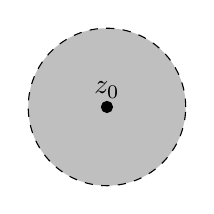
\begin{tikzpicture}

\draw[dashed, fill = lightgray] (1,0) arc (0:360:1);
\draw[fill = black] (0,0) circle (2pt);
\draw (0,0) node[inner sep = -2pt, label = {[label distance = -1pt]90:$z_0$}]{};
\end{tikzpicture}
\end{center}

Open balls are the basic building blocks of open sets. There are two equivalent characterisations:

\begin{defbo}{Open Set}{openset}\index{Topology!open set}
We say that a subset $U \subset \C$ is open if for any $z_0 \in U$, there exists a ball $B_r(z_0)$ which is contained in $U$.

Alternatively, an open set is an arbitrary union of open balls.
\end{defbo}

We can visualize this definition as:

\begin{center}
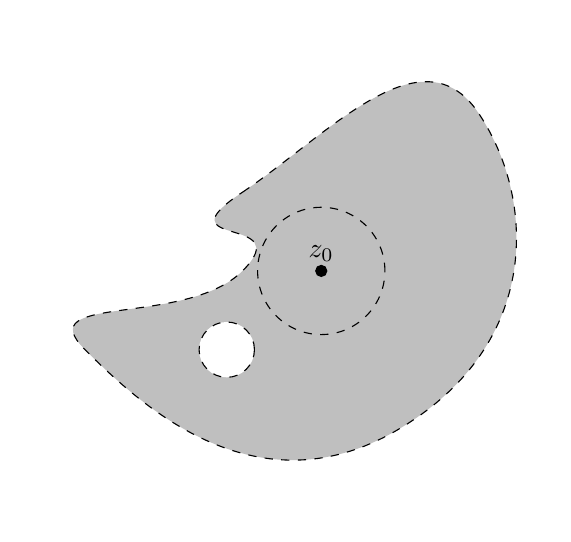
\begin{tikzpicture}
\draw[dashed, fill = lightgray] plot [smooth cycle, tension = 1.3] coordinates {(0,0)  (0,1) (3,2) (2,-2) (-2,-1)};
\draw[dashed, fill = white] (-0.2,-1) circle (10pt);

\draw[fill = black] (1,0) circle (2pt) node[inner sep = -2pt, label = {[label distance = -1pt]90:$z_0$}]{};
\draw[dashed] (1,0) circle (23pt);

\end{tikzpicture}
\end{center}

Notice that around the point $z_0$, we have found a ball $B_r(z_0)$ contained entirely in $U$, which is the shaded region. We could do the same for any point in the shaded region, if we desired.

How do we recognize open sets in practice? If we have a picture, it's easy to do so. The set shouldn't contain any ``edge". This is an intuitive notion which is easy to see visually, so we won't go through the effort of describing it formally. There is a formal definition, but it isn't very helpful for developing a visual heuristic.

Algebraically, it's much easier to determine open sets. Open sets are generally described by conditions involving inequalities of some variety. For example: $\{z\in \C| \RE(z) > 1\}$ is an open set. Open balls are open sets. $\C$ and the empty set are open. And there are many other examples.

In addition to open sets, we need one more topological notion: connectedness. The idea behind a set being "connected" is that it is in one piece. To describe this formally, we need to talk about paths.

\begin{defbo}{path}{path}\index{Topology!path}\index{path}A path $\gamma$ in $\C$ is a function $\gamma:[0,1] \rightarrow \C$ such that $\RE(\gamma)$ and $\IM(\gamma)$ are continuous functions.\end{defbo}

In a set that is in one piece, it should be possible to draw a path between two points in the set without leaving the set. And this is precisely the definition of connectedness.

\begin{defbo}{Connected Set}{connectedset}\index{Topology!connected set} A set $U\subset \C$ is called connected if for any two $z_0,z_1\in U$ there exists a path $\gamma$ such that $\gamma(0) = z_0$, $\gamma(1) = z_1$, and $\gamma(t)\in U$ for all $t$.\end{defbo}

Some examples of connected sets:

\begin{center}
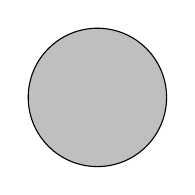
\begin{tikzpicture}[baseline=(current bounding box.center)]

\draw[fill = lightgray] (0,0) circle (25pt);

\end{tikzpicture}
\qquad or \qquad
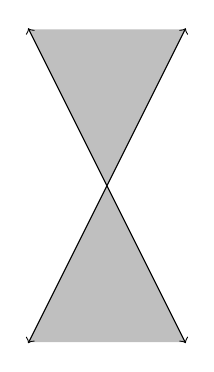
\begin{tikzpicture}[baseline=(current bounding box.center)]

\draw[fill = lightgray, <->] (-1,2) -- (0,0) -- (1,2);
\draw[fill = lightgray, <->] (-1,-2) -- (0,0) -- (1,-2);

\end{tikzpicture}
\qquad or \qquad
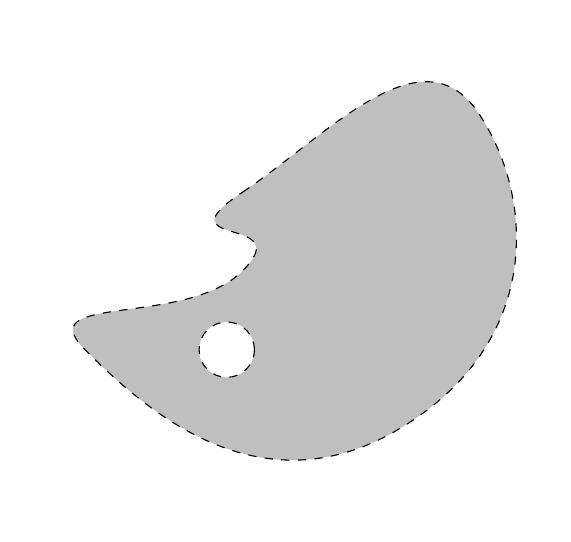
\begin{tikzpicture}[baseline=(current bounding box.center)]


\draw[dashed, fill = lightgray] plot [smooth cycle, tension = 1.3] coordinates {(0,0)  (0,1) (3,2) (2,-2) (-2,-1)};
\draw[dashed, fill = white] (-0.2,-1) circle (10pt);

\end{tikzpicture}

\end{center}

On the other hand, these are sets that are not connected:

\begin{center}
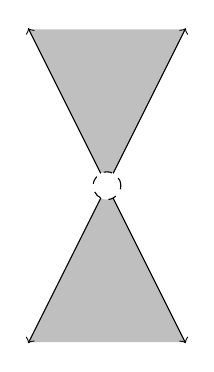
\begin{tikzpicture}[baseline=(current bounding box.center)]

\draw[fill = lightgray, <->] (-1,2) -- (0,0) -- (1,2);
\draw[fill = lightgray, <->] (-1,-2) -- (0,0) -- (1,-2);

\draw[fill = white, dashed] (0,0) circle (5pt);

\end{tikzpicture}
\qquad or \qquad
\begin{tikzpicture}[baseline=(current bounding box.center)]
\draw[fill = CORinner] (-1,0) circle (20pt);
\draw[fill = CORinner] (0,-1) -- (2,2) -- (3.5,0) -- (0,-1);
\end{tikzpicture}
\qquad or \qquad
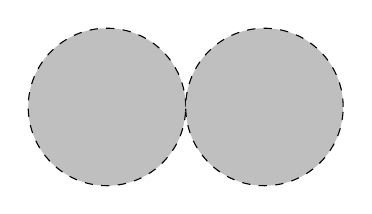
\begin{tikzpicture}[baseline=(current bounding box.center)]
\draw[fill = lightgray, dashed] (-1,0) circle (1);
\draw[fill = lightgray, dashed] (1,0) circle (1);
\end{tikzpicture}
\end{center}

The first of these is hopefully self-explanatory. It's in two pieces. The second of these, which consists of the triangle and the circle, is also in two discrete pieces.

In the third picture, we have open balls which are tangent to one another. However, since they are missing their boundaries, these two sets actually have a gap between them!

Putting these two notions together, we have the basic topological object we will be dealing with in this course:

\begin{defbo}{Domain}{domain}\index{Domain}
A set $U\subset \C$ is called a domain if it is open and connected.
\end{defbo}

\begin{note} This is not the same thing as the domain of a function! You need to be able to tell the difference from context. If we are not discussing a function, then domain will be referring to this definition. In contexts where a function is also being discussed, you will need to be vigilant. There is a difference between the language ``the domain $U$" and ``the domain $U$ of $f$."\end{note}

\begin{note} The last note, while an important technical issue, doesn't quite give the full picture.

In the context of this course, domains will almost only ever occur as the domain of a differentiable function. (In fact, what's called an "analytic function", which we will see soon.)
\end{note}

\subsection{Returning to Differentiation}

Now that we have some topological language, we can get to the point: how do we tell if a function is differentiable?

\begin{defbo}{Holomorphic or Analytic Functions}{holomorph}\index{Analytic Function}\index{Holomorphic Function}
A function $f$ is holomorphic (or analytic) on an open set $U$ if it is differentiable at each point in $U$.

A function $f$ is called holomorphic (or analytic) if it is holomorphic on its domain.
\end{defbo}

\begin{note} The textbook does not use the terminology ``holomorphic" to describe these functions. However, to be precise, analytic really means something different. An analytic function is a function that is equal to a power series.

However, it is one of the crowning achievements of complex analysis that every holomorphic function is analytic. (I.e., if $f$ is differentiable on an open set, then it can be described by power series on that open set.) As such, holomorphic and analytic are the same condition on $\C$. This is not true on $\R$ that differentiable and analytic are the same though, so it is worthwhile to make this distinction.

Plus, I just like the sound of holomorphic more.
\end{note}

So what was the point of introducing all these definitions? Do we get something out of this?

\begin{thmbo}{}{}Suppose $f = u + iv$ is defined on an open set $U$. If $u,v, u_x, u_y, v_x, v_y$ are defined and continuous everywhere in $U$ and $u,v$ satisfy the Cauchy-Riemann equations, then $f$ is holomorphic on $U$.
\end{thmbo}

\begin{proof} The proof of this requires a result from multivariable calculus:

If $u_x$ and $u_y$ are continuous, then $u$ is differentiable. This means that there exists a function $\varepsilon_u(x,y)$ such that:
$$u(x + a,y+b) = u(x,y) + au_x + bu_y  + \varepsilon_u(a,b)$$

\noin The function $\varepsilon_u$ satisfies the condition that:
$$\lim_{(a,b) \rightarrow (0,0)} \frac{\varepsilon_u(a,b)}{\sqrt{a^2 + b^2}} = 0$$

And similarly:
$$v(x + a,y+b) = v(x,y) + av_x + bv_y  + \varepsilon_v(a,b)$$

\noin where $\varepsilon_v$ is defined similarly for $v$.

As such:
\begin{align*}\lim_{a+ib \rightarrow 0} \frac{f(z + h) - f(z)}{h} &= \lim_{a+ib \rightarrow 0} \frac{u(x+a,y+b) + iv(x+a,y+b) - (u(x,y) + iv(x,y))}{a+ib}\\
&= \lim_{a+ib \rightarrow 0} \frac{au_x + bu_y + i(av_x + bv_y) + \varepsilon_u(a,b) + i\varepsilon_v(a,b)}{a+ib}\\
&= \lim_{a+ib \rightarrow 0} \frac{au_x - bv_x + i(av_x + bu_x)}{a + ib} +\lim_{a+ib \rightarrow 0} \frac{\varepsilon_u(a,b) + i\varepsilon_v(a,b)}{a+ib}\\
\end{align*}

Now, $au_x -bv_x + i(av_x + bu_x) = (a+ib)u_x + (ia - b)v_x = (a+ib)u_x + i(a+ib)v_x$. As such:
$$f'(z) = u_x + iv_x  +\lim_{a+ib \rightarrow 0} \frac{\varepsilon_u(a,b) + i\varepsilon_v(a,b)}{a+ib}$$

So we need only consider this last limit. However, note that by the triangle inequality:
$$\left|\frac{\varepsilon_u(a,b) + i\varepsilon_v(a,b)}{a+ib}\right| \le \frac{|\varepsilon_u(a,b)|}{\sqrt{a^2 + b^2}} + \frac{|\varepsilon_v(a,b)|}{\sqrt{a^2 + b^2}}$$

By the definition of $\varepsilon_u$ and $\varepsilon_v$, we know that:
$$\lim_{(a,b)\rightarrow (0,0)} \frac{|\varepsilon_u(a,b)|}{\sqrt{a^2 + b^2}} + \frac{|\varepsilon_v(a,b)|}{\sqrt{a^2 + b^2}} = 0$$

So by the squeeze theorem, $\lim_{a+ib \rightarrow 0} \frac{\varepsilon_u(a,b) + i\varepsilon_v(a,b)}{a+ib} = 0$ as well.

As such, $f'(z) = u_x + iv_x$, and $f$ is differentiable at $z$. Since this applies for any $z\in U$, we see that $f$ is holomorphic on $U$.
\end{proof}


\begin{ex}{}{} Show that $e^z$ is analytic on $\C$.

We need to write $e^z$ as $u + iv$, and show that $u,v, u_x, u_y, v_x, v_y$ are continuous. We also need to show that $u,v$ satisfy the Cauchy-Riemann equations.

To start, $e^z = e^{x}e^{iy} = e^x\cos(y) + ie^x\sin(y)$. As such, $u(x,y) = e^x\cos(y)$ and $v(x,y) = e^x\sin(y)$. These are continuous.

We compute the partials:
$$u_x = e^x\cos(y)$$
$$u_y = -e^x\sin(y)$$
$$v_x = e^x\sin(y)$$
$$v_y = e^x\cos(y)$$


Notice that these are all continuous. And further, that:
$$u_x = e^x\cos(y) = v_y$$
$$u_y = -e^x\sin(y) = -v_x$$

As such, $e^z$ satisfies the conditions of the theorem, and is therefore analytic on $\C$.
\end{ex}